\documentclass{standalone}
\begin{document}
\subsubsection{U-Net}
The U-net is a convolutional network architecture for fast and precise segmentation of images especially in the biomedical field\cite{unet}.
One of the main advantage of the U-net is the ability of dealing with small dataset. 
The name U-net refers to the U shape of the network architecture. 
The whole U-net structure, showed in Figure\ref{fig:unet}, can be split into two main parts:

\paragraph{Encoder:}
or \textit{contraction path} is a sequence of convolutional and max pooling layers with the aim of extracting features and reducing dimensionality.

\paragraph{Decoder:}
or \textit{expansion path} is a sequence of transpose convolutional layers with the aim of reconstructing the feature map and consequently the segmentation mask.
\\
The \textit{Encoder} is a typical Convolutional Neural Network that consists in the repeated application of convolutions, followed by ReLu activation function and max pooling operations.
During the contraction the input size is decreased and so the spatial information, while the information about features is increased.
The \textit{Decoder} combines the feature maps and the spatial information by a sequence of transpose convolutions (or up-convolutions) and concatenations with the features from the contracting path (grey arrows in Figure\ref{fig:unet}).
\begin{figure}[ht]

    \centering
    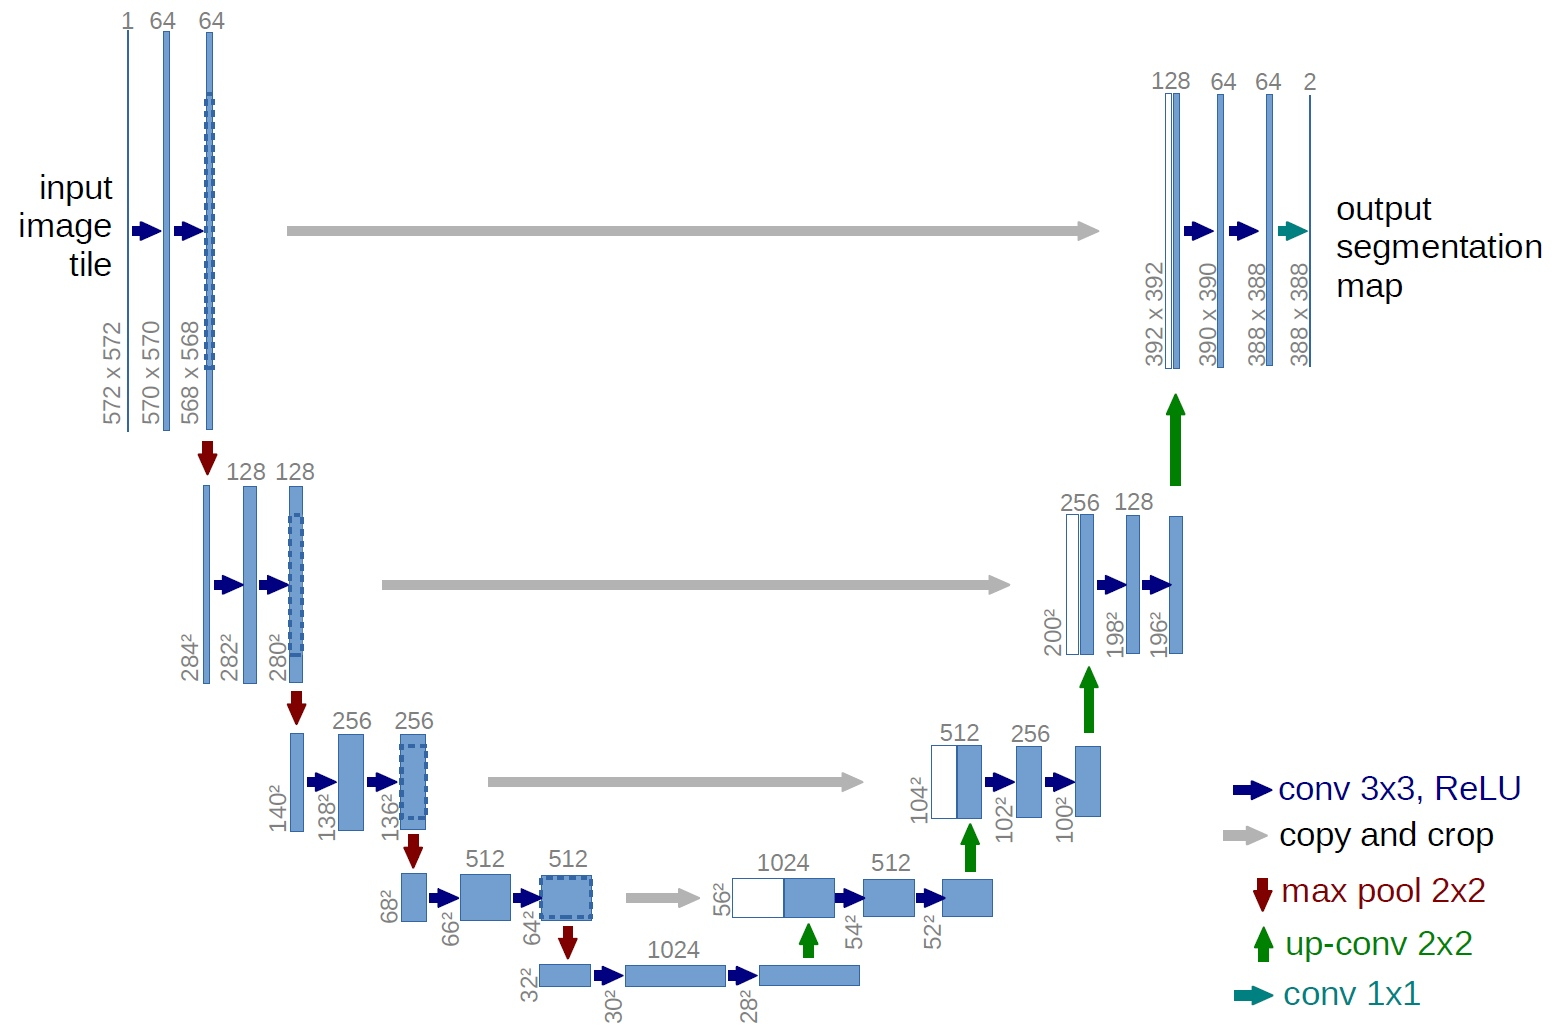
\includegraphics[width=.85\textwidth]{../images/U-Net arch.jpeg}
    
    \caption{Original U-Net architecture. We can notice the U-shape made by the expansion and contraction path. Each blue box corresponds to a series of feature maps. White boxes represent copied feature maps. The arrows denote the different operations. From \textit{U-Net: Convolutional Networks for Biomedical Image Segmentation}\cite{unet}.}
    \label{fig:unet}
    
    \end{figure}

\end{document}